% !TEX root = ../main.tex

%%%%%%%%%%%%%%%%%%%%%%%%%%%%%%%%%%%%%%%%%
% ZHAW BEAMER
% section
% 
% Authors:
% Martin Oswald
%%%%%%%%%%%%%%%%%%%%%%%%%%%%%%%%%%%%%%%%%

%----------------------------------------
%   SECTION TITLE
%----------------------------------------
\section{Why \LaTeX}
\label{sec:introduction}
\frame[plain]{\sectionpage}


%----------------------------------------
%   SECTION CONTENT
%----------------------------------------
\begin{frame}{Why \LaTeX}
    \begin{itemize}
        \item<1-> Best for typesetting technical content: figures, equations ($E=mc^2!$), tables, etc.,
        \item <2->Have to cite a lot of references? No worries! \LaTeX can automate to suite your chosen style. 
        \item <3->Can easily produce table of contents, indexes, list of figures etc. with a single command \textbackslash\textit{tableofcontents} 
        \item<4-> Can facilitate version control and also suitable for collaboration (Git users!)
        \
    \end{itemize}
\end{frame}

%----------------------------------------
%   SECTION TITLE
%----------------------------------------
\section{Getting started with \LaTeX}
\label{sec:introduction}
\frame[plain]{\sectionpage}


%----------------------------------------
%   SECTION CONTENT
%----------------------------------------
\begin{frame}{How to get started?}
    \begin{itemize}
        \item<1-> Local installation in your computer 
        \begin{itemize}
            \item TeXMaker, TeXStudio, TeXWorks, MiTeX..... 
        \end{itemize}
         \vspace{5em}
        \item <2-> Or you can skip all that and use \textcolor{red}{Overleaf}
        \begin{itemize}
            \item \href{https://www.overleaf.com/}{https://www.overleaf.com/}
            \item Free account for single user
        \end{itemize}
        
    \end{itemize}
\end{frame}

%----------------------------------------
%   SECTION TITLE
%----------------------------------------
\section{Document structure}
\label{sec:structure}
\frame[plain]{\sectionpage}


%----------------------------------------
%   SECTION CONTENT
%----------------------------------------
\begin{frame}{Document writing}
    \begin{itemize}
        \item<1-> Creating title, author, affiliations
        \item <2-> Sections, subsections, subsubsections
        \item <3-> Labeling the sections to refer to them again
        \item <4-> Table of contents
        \item <5-> Font sizes, colors, page layouts
    \end{itemize}
\end{frame}

\begin{frame}[fragile]{Basic Syntax: Creating a document}
\begin{itemize}
    \item Everything that begins.. ends!
\end{itemize}
\begin{verbatim}
%    \documentclass[12pt,a4paper]{article} 
% creates an article on a4 size with 12 pt. font size 
%    \begin{document} % need begin and end while creating the document
%    \end{document}
\end{verbatim}
\end{frame}

\begin{frame}[fragile]{Basic Syntax: Creating a document}
\begin{itemize}
    \item Everything that begins.. ends!
\end{itemize}
\begin{verbatim}
%    \documentclass[12pt,a4paper]{article} 
%    \title{Typesetting with \latex}
%    \author{Vedasri Godavarthi}
%    \begin{document} % need begin and end while creating the document
%    \maketitlepage
%         Content appears here
%    \end{document}
\end{verbatim}
\end{frame}

\begin{frame}[fragile]{Margins, sections, subsections...}
\begin{itemize}
    \item Everything that begins.. ends!
\end{itemize}
\begin{verbatim}
%    \documentclass[12pt,a4paper]{article} 
%    \usepackage[margin=1in]{geometry}
%    \title{Typesetting with \latex}
%    \author{Vedasri Godavarthi}
%    \begin{document} 
%    \maketitlepage
%    \section{Section 1}
%    \subsection{Subsection 1.1}
%    \section*{Section without numbering}
%    \subsection*{Subsection without numbering}
%    \end{document}
\end{verbatim}
\end{frame}

\begin{frame}[fragile]{Font colors, styles}
\begin{itemize}
    \item Everything that begins.. ends!
\end{itemize}
\begin{verbatim}
%    \section{Section : Font fomatting}
%    \subsection{Subsection : Colors}
%    \textcolor{red}{this is red}
%    \textcolor{blue}{Let's make this blue}
%    \subsection{Subsection : Styles}
%    \textbf{This is red}
%    \textit{Let's make this italic}
%    \textbf{\textit{Italic and Bold}}
%    \section*{Section without numbering}
%    \subsection*{Subsection without numbering}
\end{verbatim}
\end{frame}


%----------------------------------------
%   SECTION TITLE
%----------------------------------------
\section{Equations}
\label{sec:equations}
\frame[plain]{\sectionpage}


%----------------------------------------
%   SECTION CONTENT
%----------------------------------------

\begin{frame}[fragile]{Equations}

\begin{equation*}
f(x) = \frac{1}{2\pi} \int_{-\infty}^{\infty} e^{-ix\xi} \left(1 + \frac{\sin(\xi)}{\xi}\right) \, d\xi \footnote{I asked ChatGPT: Example of most complicated equation in latex}
\label{eq:complicated_eqn}
\end{equation*}
    \begin{itemize}
        \item<1-> Ease of embedding complicated equations in a text.
        \item<2-> What should we do? 
        \begin{verbatim}
            \begin{?}..\end{?}
        \end{verbatim}
        \end{itemize}
 
\end{frame}

\begin{frame}[fragile]{Equations}
%\vspace{-5em}
\begin{equation*}
f(x) = \frac{1}{2\pi} \int_{-\infty}^{\infty} e^{-ix\xi} \left(1 + \frac{\sin(\xi)}{\xi}\right) \, d\xi \footnote{I asked ChatGPT: Example of most complicated equation in latex}
\label{eq:complicated_eqn}
\end{equation*}
    \begin{itemize}
        \item Ease of embedding complicated equations in a text.
        \item What should we do? 
        \begin{verbatim}
            \begin{equation} < Place equation here >\end{equation}
        \end{verbatim}
        \item<3-> Inline: \begin{verbatim} $$ <Equation $$\end{verbatim}
        \item<4-> Multiple equations: \begin{verbatim}
            \begin{align} x&=1\\ y&=2\\ x+y &=3 \end{align}
        \end{verbatim}
        \end{itemize}
\end{frame}
%----------------------------------------
%   SECTION TITLE
%----------------------------------------
\section{Figures}
\label{sec:equations}
\frame[plain]{\sectionpage}


%----------------------------------------
%   SECTION CONTENT
%----------------------------------------
\begin{frame}{Figures}
\vspace{-2em}
    \begin{figure}[t!]
    \centering
    \begin{subfigure}[t]{0.5\textwidth}
        \centering
        
\includegraphics[width=0.5\textwidth]{sections/begin_figure_meme.png}
        \caption{Small Meme}
    \end{subfigure}%
    ~ 
    \begin{subfigure}[t]{0.5\textwidth}
        \centering
        
\includegraphics[width=0.8\textwidth]{sections/begin_figure_meme.png}
        \caption{Large Meme}
    \end{subfigure}
    \caption{\LaTeX\: meme}
    \label{fig:meme}
\end{figure}
\end{frame}

%----------------------------------------
%   SECTION CONTENT
%----------------------------------------
\begin{frame}[fragile]{Figures: Background}
\begin{itemize}
    \item Let's look at the syntax
\end{itemize}
\begin{verbatim}
    \begin{?} <Details> \end{?}
\end{verbatim}
\end{frame}

%----------------------------------------
%   SECTION CONTENT
%----------------------------------------
\begin{frame}[fragile]{Figures: Background}
\begin{itemize}
    \item Let's look at the syntax
\end{itemize}
\begin{verbatim}
    \begin{figure} 
    \centering % Justification
    \includegraphics[width=0.8\textwidth]{fig.png} 
    % includes graphics with 80% textwidth
    %\includegraphics[height=]%includegraphics[scale=]
    \caption{Meme} %caption
    \label{fig:meme} % can refer to figure in the text using this label
    \end{figure}
\end{verbatim}
\end{frame}

%----------------------------------------
%   SECTION CONTENT
%----------------------------------------
\begin{frame}[fragile]{Figures: Subfigures}
\begin{itemize}
    \item Packages: \textbf{subcaption}, \textbf{graphicx} and we add these before \textbackslash begin\{document\}
    \item \textbf{\textbackslash usepackage\{subcaption\}}
\end{itemize}
\begin{columns}
    \begin{column}{0.5\textwidth}
    \textbf{First subfigure}
        \begin{small}
\begin{verbatim}
     \begin{figure}[t!]
    \centering
    \begin{subfigure}[t]{0.5\textwidth}
        \centering
        \includegraphics[width=]{fig.png}
        \caption{Small Meme}
    \end{subfigure}%
    \end{verbatim}
    \end{small}
    \end{column}
\begin{column}{0.5\textwidth}
\textbf{Second subfigure}
        \begin{small}
\begin{verbatim}
    \begin{subfigure}[t]{0.5\textwidth}
        \centering
        \includegraphics[width=]{fig.png}
        \caption{Large Meme}
    \end{subfigure}
    \caption{\LaTeX\: meme}
\end{figure}
\end{verbatim}
\end{small}
\end{column}
\end{columns}
\end{frame}
%----------------------------------------
%   SECTION TITLE
%----------------------------------------
\section{Cross referencing}
\label{sec:referencing}
\frame[plain]{\sectionpage}

%----------------------------------------
%   SECTION CONTENT
%----------------------------------------
\begin{frame}[fragile]{Cross referencing}
\begin{itemize}
    \item<1-> Cross referencing is important when referring to equations, tables, figures etc., in the text.
    \item<2-> The readers can point to eq.(2) instead to writing it again.
    \item<3-> We use \textttt{\textbackslash label} and \textttt{\textbackslash ref}, such as \textttt{\textbackslash label\{fig:meme\}} to label inside \texttt{\textbackslash begin\{figure\}..} and in the text as \textttt{\textbackslash ref\{fig:meme\}} to refer to Fig.~\ref{fig:meme}.
\end{itemize}
\begin{columns}
    \begin{column}{0.4\textwidth}
    \textbf{Labeling figure}
           \begin{small}
         \begin{verbatim}
    \begin{figure} 
    \centering 
    \includegraphics{fig.png} 
    \caption{Meme} %caption
    \label{fig:meme} %label
    \end{figure}
    \end{verbatim}
    \end{small}  
    \end{column}
       \begin{column}{0.4\textwidth}
       \textbf{Labeling equation}
           \begin{small}
         \begin{verbatim}
    \begin{equation} 
    E=mc^2
    \label{eq:energy_mass} %label
    \end{equation}
    \end{verbatim}
    \end{small}  
    \end{column}
\end{columns}
  
\end{frame}

%----------------------------------------
%   SECTION TITLE
%----------------------------------------
\section{External citations}
\label{sec:referencing}
\frame[plain]{\sectionpage}
%----------------------------------------
%   SECTION CONTENT
%----------------------------------------
\begin{frame}{References: External}
 \begin{itemize}
     \item Use any source of citations: Google scholar, Mendeley, journal
     \item We obtain the bibtex from the above locations.
     \item Place them in a .bib file, say references.bib and we can use it cite.
 \end{itemize}
 \begin{figure}
     \centering
     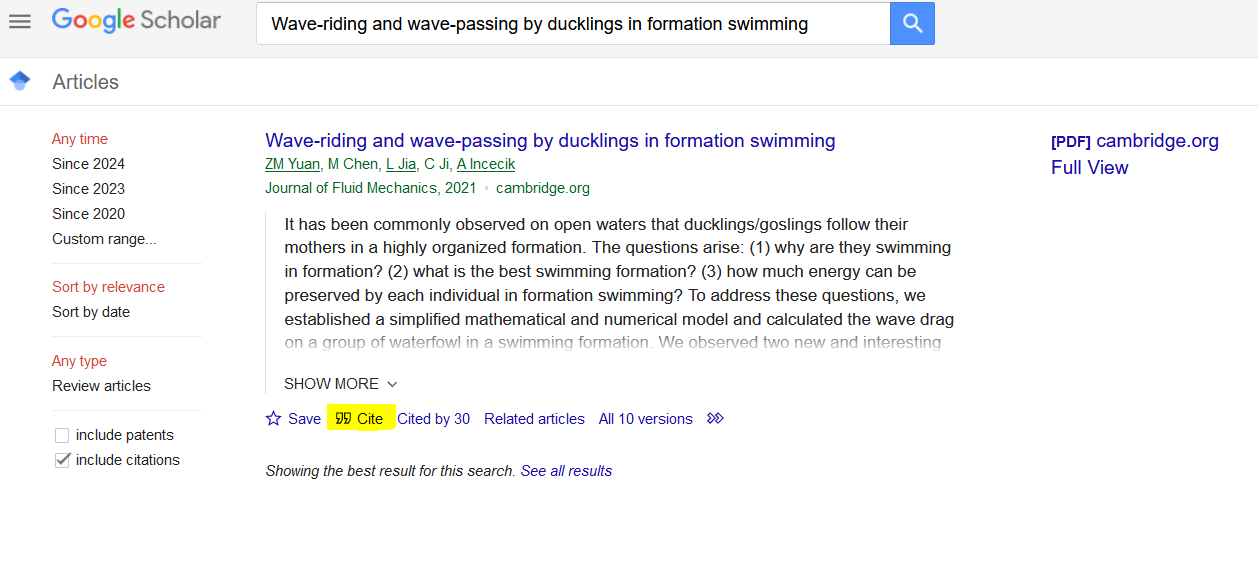
\includegraphics[width=0.6\textwidth]{sections/citation01.PNG}
     \caption{Search in google scholar}
     \label{fig:cite_step01}
 \end{figure}
\end{frame}

%----------------------------------------
%   SECTION CONTENT
%----------------------------------------
\begin{frame}{References: External}
 \begin{itemize}
     \item Use any source of citations: Google scholar, Mendeley, journal
     \item We obtain the bibtex from the above locations.
     \item Place them in a .bib file, say references.bib and we can use it cite.
 \end{itemize}
 \begin{figure}
     \centering
     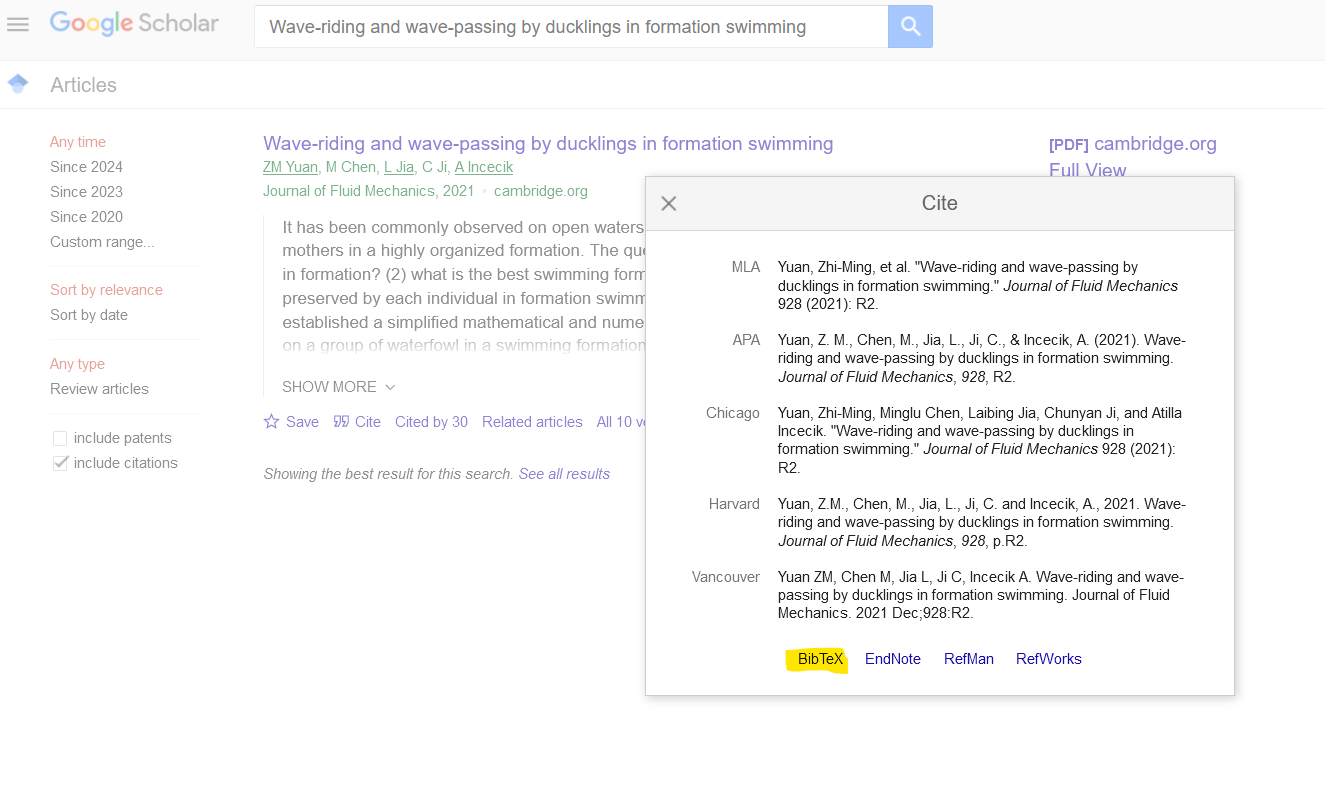
\includegraphics[width=0.5\textwidth]{sections/citation02.PNG}
     \caption{Citation formats}
     \label{fig:cite_step01}
 \end{figure}
\end{frame}

%----------------------------------------
%   SECTION CONTENT
%----------------------------------------
\begin{frame}{References: External}
 \begin{itemize}
     \item Use any source of citations: Google Scholar, Mendeley, journal
     \item We obtain the BibTeX from the above locations.
     \item Place them in a .bib file, say references. bib and we can use it cite.
 \end{itemize}
 \begin{figure}
     \centering
     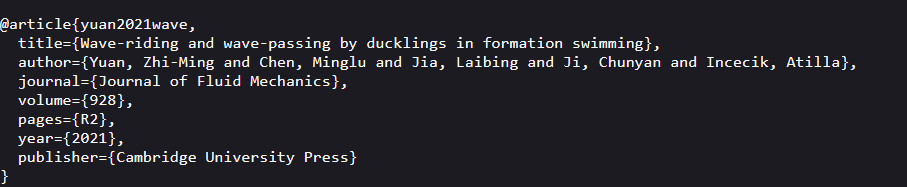
\includegraphics[width=0.6\textwidth]{sections/citation03.PNG}
     \caption{.bib file $\rightarrow$ copy and paste this in .bib}
     \label{Bibtex}
 \end{figure}
  \begin{itemize}
     \item<1-> This reference can be cited as \textttt{\textbackslash cite\{yuan2021wave\}} \cite{yuan2021wave}.
 \end{itemize}
 \end{frame}